\documentclass[conference]{IEEEtran}
% DATA 245 final project report. Compile with pdfLaTeX (Overleaf: upload this folder, main file main.tex).
\usepackage{cite}
\usepackage{amsmath,amssymb}
\usepackage{graphicx}
\usepackage{booktabs}
\usepackage{multirow}
\usepackage{url}
\usepackage[hidelinks]{hyperref}
\graphicspath{{figures/}}
% Let LaTeX place more figures per page so they stay close to the text that discusses them.
\setcounter{topnumber}{3}
\setcounter{dbltopnumber}{2}
\renewcommand{\topfraction}{0.9}
\renewcommand{\dbltopfraction}{0.9}
\renewcommand{\textfraction}{0.1}
\renewcommand{\floatpagefraction}{0.8}
\renewcommand{\dblfloatpagefraction}{0.8}

\begin{document}

\title{Evaluating Classical Machine Learning Robustness Under Data Drift: A Comparative Study of Retraining Strategies}

\author{
\IEEEauthorblockN{Uday Patel}
\IEEEauthorblockA{San Jos\'e State University\\San Jos\'e, CA, USA}
\and
\IEEEauthorblockN{Tanya Shah}
\IEEEauthorblockA{San Jos\'e State University\\San Jos\'e, CA, USA}
\and
\IEEEauthorblockN{Rutuja Saste}
\IEEEauthorblockA{San Jos\'e State University\\San Jos\'e, CA, USA}
\and
\IEEEauthorblockN{Himja Patel}
\IEEEauthorblockA{San Jos\'e State University\\San Jos\'e, CA, USA}
}

\maketitle

\begin{abstract}
A model trained on past data may become less useful as the data it sees changes. Retraining on a fixed schedule can waste effort, while waiting too long can hurt predictions. We asked whether drift-triggered retraining, which retrains only when the Population Stability Index (PSI) of an input crosses an alert threshold, maintains predictive performance better than never retraining (static) or retraining on a fixed schedule (periodic). Using the chronologically ordered UCI Bank Marketing dataset (41,188 calls, 11.3\% subscriptions), we built a leakage-reviewed pipeline, compared four classical models, monitored drift with PSI and the Kolmogorov--Smirnov (KS) statistic, and ran all three strategies through one shared loop on a real chronological replay and three controlled synthetic scenarios. On the real replay, the three strategies were practically indistinguishable for Logistic Regression (mean precision--recall area under the curve, PR-AUC, of 0.399, 0.400 and 0.400 against a random baseline of 0.308), while, in this single run, retraining lifted a weaker linear support vector machine (SVM) to about the same level. Drift-triggered retraining retrained twice as often as periodic retraining without additional benefit, because its alarm fired in every real window. In synthetic scenarios the alarm detected shifts promptly with no false alarms, but the static model's performance did not measurably drop after the detected shifts. Diagnostics are consistent with weak predictive signal, rather than model staleness, being the main limitation, though they cannot rule out gains from more recent data. We also found and corrected a row-reuse flaw in our first synthetic design that likely inflated the apparent benefit of retraining (the original and corrected designs differ in more than one factor).
\end{abstract}

\begin{IEEEkeywords}
concept drift, data drift, model retraining, population stability index, imbalanced classification, bank marketing
\end{IEEEkeywords}

%======================================================================
\section{Introduction}

Training a model is only one part of a machine learning system. In practice the data keeps changing: customers change, campaigns change and the economy changes. A model that performs well today may perform worse later, a problem known as data drift or concept drift~\cite{gama2014survey,lu2019review}. The usual response is to retrain, but retraining raises its own question: \emph{when} should a model be retrained? Retraining too often wastes computation and engineering effort; waiting too long may let prediction quality decline.

When our team first discussed project ideas, we considered fraud detection and failures in multi-agent AI systems. Both were interesting, but we wanted a question that was manageable within one semester while still addressing a real machine learning problem. Data drift stood out because it forced us to think beyond ``train once and report accuracy'' and to study how a model behaves over time. We also liked that the question could be tested experimentally, by comparing three ways of maintaining a model.

\textbf{Research question.} \emph{When data changes over time, can drift-triggered retraining maintain better predictive performance than static or periodically retrained classical machine learning models?}

Our starting hypothesis was that drift-triggered retraining would give a better balance between predictive performance and computational cost: by retraining only when the data changed meaningfully, it might match a fixed schedule with fewer retraining events. As Section~\ref{sec:results} shows, that is not what we observed, and understanding why became the most valuable part of the project.

\textbf{Contributions.} (1) A leakage-reviewed, chronologically ordered evaluation pipeline for the UCI Bank Marketing data, with every assumption recorded. (2) A comparison of four classical models and an economic-feature sensitivity test. (3) One shared experiment loop that compares static, periodic and drift-triggered retraining on a real chronological replay and three controlled scenarios under identical rules. (4) Diagnostics that explain why the strategies performed alike, and (5) the detection and correction of a data-reuse flaw in our own synthetic design.

%======================================================================
\section{Related Work}

\textbf{Concept drift.} Gama \emph{et~al.}~\cite{gama2014survey} survey adaptation methods and distinguish ``blind'' updating on a schedule from ``informed'' updating triggered by a change detector, the two families compared in this project. Lu \emph{et~al.}~\cite{lu2019review} review drift detection, understanding and adaptation, and Webb \emph{et~al.}~\cite{webb2016characterizing} formalize kinds of drift. We follow the common distinction between covariate drift (the input distribution changes), prior or label drift (the share of each class changes) and concept drift (the relationship between inputs and outcome changes).

\textbf{Drift statistics.} The two-sample KS statistic~\cite{massey1951ks} is the largest gap between two cumulative distributions. The PSI, widely used in credit-risk monitoring~\cite{siddiqi2006credit}, compares the share of observations per bin between a reference and a current sample, with 0.1 and 0.25 as conventional ``moderate'' and ``major'' shift thresholds. Both describe input change; neither measures model performance directly.

\textbf{Evaluation and leakage.} For imbalanced problems the precision--recall curve is more informative than the ROC curve~\cite{saito2015pr}, motivating PR-AUC as our primary metric. Kaufman \emph{et~al.}~\cite{kaufman2012leakage} describe how information unavailable at prediction time can inflate results; this guided our leakage review. The dataset was introduced by Moro \emph{et~al.}~\cite{moro2014data}; its documentation~\cite{uci2014bank} advises discarding call duration for realistic prediction.

%======================================================================
\section{Dataset and Exploratory Analysis}
\label{sec:data}

We use \texttt{bank-additional-full.csv} from the UCI repository~\cite{uci2014bank,moro2014data}: 41,188 telemarketing calls by a Portuguese bank, with 20 inputs and a binary target (term-deposit subscription). The file is documented as ordered by date from May~2008 to November~2010 but has no date column, so we describe time by row position. We chose this dataset for three reasons: its chronological order, which our question depends on; real campaign data with customer, previous-campaign and economic features; and a period of strong economic change, although we do not attribute any observed change to a specific economic event.

Only 11.3\% of rows are ``yes'' (4,640 vs.\ 36,548, about 7.9:1), so accuracy is misleading. There are no true missing values, but six categorical columns use ``unknown'' (20.9\% of \texttt{default}), 12 rows are exact duplicates, and \texttt{pdays}~=~999, a sentinel value (not a number of days) that the documentation reads as ``not previously contacted'' but that we do not assume always means that (assumption A3), appears in 96.3\% of rows.

Comparing the first 70\% of rows with the last 30\% (an illustrative cut, not our modeling split), the subscription rate rises from 5.6\% to 24.6\%. All five economic indicators shift strongly (KS 0.59--1.00; PSI 4.48--11.52), while \texttt{age} and \texttt{campaign} shift little (KS 0.095 and 0.090; PSI 0.12 and 0.05) (Fig.~\ref{fig:eda}). The large PSI values for economic indicators depend on binning and an empty-bin floor, so we only claim that they are far above 0.25. These shifts motivated the study, but they do not by themselves show that any model degrades.

\begin{figure*}[t]
\centering
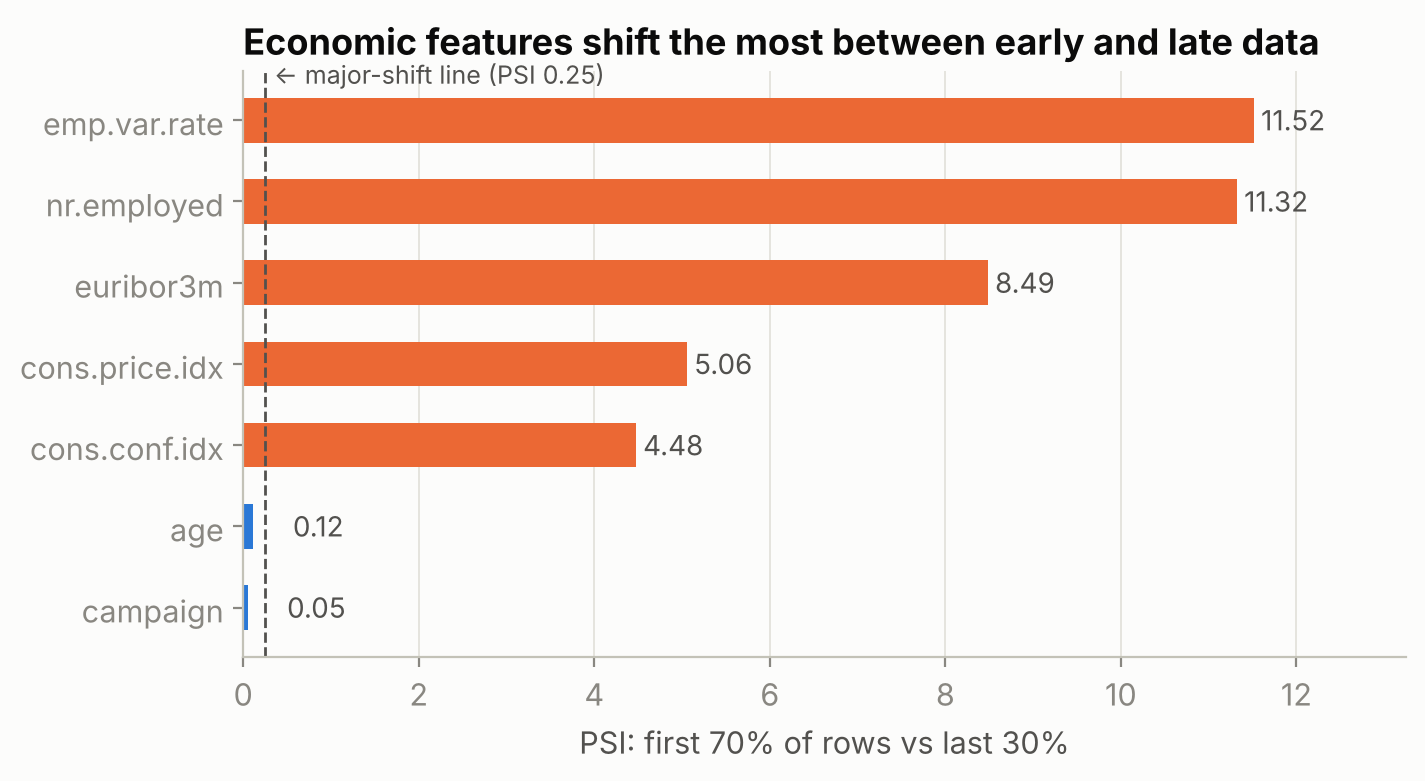
\includegraphics[width=0.7\textwidth]{figures/04_early_vs_late_psi.png}
\caption{PSI between the first 70\% and last 30\% of rows (illustrative cut). Economic indicators shift far more than the customer features tested.}
\label{fig:eda}
\end{figure*}

%======================================================================
\section{Prediction Task, Leakage Review and Assumptions}
\label{sec:leakage}

\textbf{Prediction moment.} We predict whether a customer will subscribe \emph{immediately before a planned marketing call begins}. Only information available before dialing may be used. Call \texttt{duration} is therefore excluded: it is known only after the call and strongly reveals the outcome~\cite{uci2014bank}.

\textbf{Feature groups.} We reviewed all 19 remaining inputs against the UCI documentation (Table~\ref{tab:features}). Customer attributes and previous-campaign history are provisionally available before the call. For the current-contact features and the economic indicators, the documentation does not establish whether values were known before the modeled call or when indicators were published, so their availability is unresolved. Our experiments therefore use the 10 provisionally available features.

\begin{table}[t]
\caption{Feature groups and availability before the call}
\label{tab:features}
\centering
\footnotesize
\begin{tabular}{@{}p{2.3cm}p{3.2cm}p{2.1cm}@{}}
\toprule
Group & Columns & Status \\
\midrule
Customer (7) & age, job, marital, education, default, housing, loan & Provisionally available (used) \\
History (3) & pdays, previous, poutcome & Provisionally available (used) \\
Current contact (4) & campaign, contact, month, day\_of\_week & Unresolved (not used) \\
Economic (5) & emp.var.rate, cons.price.idx, cons.conf.idx, euribor3m, nr.employed & Unresolved (sensitivity test only) \\
Duration (1) & duration & Excluded (post-call) \\
\bottomrule
\end{tabular}
\end{table}

\textbf{Assumptions.} We state our modeling assumptions explicitly: (A1) rows are in chronological order, as documented, and row order is never shuffled; (A2) customer and history features reflect information captured before the call; (A3) \texttt{pdays}~=~999 is a sentinel rather than a number of days (4,110 rows have \texttt{previous}~$>$~0 with \texttt{pdays}~=~999, so we do not assume it always means ``never contacted'' and keep those rows); (A4) ``unknown'' is a genuine category; (A5) the true outcome of a call becomes available one window later (label delay); and (A6) in synthetic scenarios, the labels that arrive for a window are a fresh sample from that window's distribution.

%======================================================================
\section{Methods: Split, Preprocessing and Models}
\label{sec:models}

\textbf{Chronological split.} The 41,188 rows are split in original order into training (first 60\%, 24,712 rows, 4.81\% ``yes''), development (next 20\%, 8,238 rows, 11.07\% ``yes'') and a reserved stream (last 20\%, 8,238 rows). The stream was not used for the initial preprocessing, fitting, tuning or model selection; in the retraining experiment its windows enter training only after their labels become available (Section~\ref{sec:strategies}).

\textbf{Preprocessing.} One scikit-learn~\cite{pedregosa2011sklearn} pipeline is fitted on training rows only: \texttt{age} is standardized; \texttt{pdays} is replaced by an indicator \texttt{pdays\_is\_999} and the real value (median-imputed from training rows); categoricals are one-hot encoded with ``unknown'' as its own category. This gives 40 model columns. Because only 6 training rows have a real \texttt{pdays} value, \texttt{pdays} and \texttt{previous} are not standardized, which avoids extreme scaled values later in time.

\textbf{Model comparison.} We compared Logistic Regression, Decision Tree, Random Forest and a Linear Support Vector Machine (SVM), each with two configurations selected on the last 20\% of the training rows, then refitted on all training rows and scored on the development rows (Table~\ref{tab:models}), reporting PR-AUC, the area under the receiver operating characteristic curve (ROC-AUC) and the F1 score. Each model was also run with the five economic indicators added as a sensitivity test. The decision threshold was chosen as the one maximizing F1 on the development rows, so the threshold-based metrics in Table~\ref{tab:models} are optimistic.

\begin{table}[t]
\caption{Development-set model comparison (random PR-AUC = 0.111)}
\label{tab:models}
\centering
\footnotesize
\setlength{\tabcolsep}{3pt}
\begin{tabular}{@{}llccc@{}}
\toprule
Features & Model & PR-AUC & ROC-AUC & F1$^\dagger$ \\
\midrule
\multirow{4}{*}{Baseline 10} & Logistic Regression & \textbf{0.179} & \textbf{0.606} & 0.244 \\
 & Linear SVM & 0.162 & 0.576 & 0.228 \\
 & Random Forest & 0.134 & 0.562 & 0.217 \\
 & Decision Tree & 0.127 & 0.558 & 0.211 \\
\midrule
\multirow{4}{*}{+ 5 economic} & Random Forest & 0.116 & 0.534 & 0.206 \\
 & Decision Tree & 0.104 & 0.471 & 0.199 \\
 & Linear SVM & 0.095 & 0.459 & 0.205 \\
 & Logistic Regression & 0.094 & 0.465 & 0.209 \\
\bottomrule
\multicolumn{5}{@{}p{\columnwidth}@{}}{\scriptsize $^\dagger$Threshold tuned on the same development rows. Predicting ``yes'' for everyone gives F1 = 0.199.}
\end{tabular}
\end{table}

Two results shaped the experiment. First, the models are weak: the best development PR-AUC (Logistic Regression, 0.179) improves only slightly on our midterm untuned baseline (0.173). Second, adding economic indicators made \emph{every} model worse, and for three models PR-AUC fell below the random baseline. A plausible explanation, which we did not test directly, is that these indicators take values in later periods far outside their training range. Together with their unresolved availability, this led us to exclude them. We shortlisted Logistic Regression and Linear SVM (both with balanced class weights) on the 10 baseline features for the retraining experiment. This also responds to teaching assistant (TA) feedback that a fixed 0.5 threshold had produced zero ``yes'' predictions at the midterm: thresholds are now tuned and reported with confusion counts (Table~\ref{tab:confusion}). At its tuned threshold, Logistic Regression finds 352 of the 912 development subscribers while flagging 1,978 customers in total.

\begin{table}[t]
\caption{Development confusion counts at the F1-tuned threshold}
\label{tab:confusion}
\centering
\footnotesize
\setlength{\tabcolsep}{3pt}
\begin{tabular}{@{}lcccccc@{}}
\toprule
Model & TP & FP & FN & TN & Precision & Recall \\
\midrule
Logistic Regression & 352 & 1,626 & 560 & 5,700 & 0.178 & 0.386 \\
Linear SVM & 363 & 1,913 & 549 & 5,413 & 0.160 & 0.398 \\
\bottomrule
\multicolumn{7}{@{}p{\columnwidth}@{}}{\scriptsize TP = subscribers found; FP = wrong ``yes'' predictions; 912 subscribers in 8,238 rows.}
\end{tabular}
\end{table}

%======================================================================
\section{Methods: Drift Detection and Scenarios}
\label{sec:drift}

\textbf{Drift measures.} For a feature with bins $i$, reference shares $r_i$ and current shares $c_i$,
\begin{equation}
\mathrm{PSI} = \sum_i (c_i - r_i)\,\ln\frac{c_i}{r_i}.
\end{equation}
Numeric features use 10 quantile bins taken from the reference sample only; categorical features and numbers with at most 10 distinct values use one bin per value; empty bins receive a floor of $10^{-4}$. The KS statistic is reported as an effect size for numeric features. We do not use its p-value, because with thousands of rows almost any difference is statistically significant.

\textbf{Trigger rule.} The model is retrained when any of the 10 model-input features has PSI~$>$~0.25 relative to the rows the current model was trained on. Economic indicators are monitored and logged separately but do not trigger retraining. To check the threshold without touching the stream, we compared 200 random samples of 1,030 training rows with all training rows: the largest PSI was 0.026 and the rule never fired.

\textbf{Scenarios.} Each strategy runs on four streams of 8 windows of about 1,030 rows (Table~\ref{tab:scenarios}). The real replay is the reserved stream in original order; it has no known change point. The synthetic scenarios are controlled experiments built from training rows: the stationary scenario has no change, and the sudden and gradual scenarios draw rows with probability proportional to $\exp(z_{\text{age}})$ (older customers more often), giving a covariate shift in a model input with a known start. Whole rows are resampled, so each customer's outcome given their features is unchanged; only the mix of customers changes.

\begin{table}[t]
\caption{Scenarios (8 windows of about 1,030 rows each)}
\label{tab:scenarios}
\centering
\footnotesize
\begin{tabular}{@{}p{1.6cm}p{6.2cm}@{}}
\toprule
Scenario & Construction and purpose \\
\midrule
Real replay & Last 20\% of rows in original order; real change, no known change point \\
Stationary & All windows from one fixed pool; counts false alarms and needless retrains \\
Sudden & Age-weighted sampling from window 5; detection delay with known change \\
Gradual & Same shift growing from window 3 to full strength at window 7 \\
\bottomrule
\end{tabular}
\end{table}

\textbf{Correcting a row-reuse flaw.} Our first synthetic design drew every window with replacement from a single pool of about 4,900 training rows. Because retraining uses earlier windows, the same rows could appear in a model's retraining history and in a window it was later scored on. We measured the overlap: for seed 42, 18\% of the rows scored in window 3 were already in the retraining history, rising to 71--80\% by window 8. This gave retrained models an unfair advantage over the static model. In the corrected design (v2), the training rows are split at random into three disjoint parts: 60\% to fit the initial model, a 20\% scoring pool from which scored windows are drawn, and a 20\% history pool from which each window's labeled copy for retraining is drawn with the same shift weights. A unit test confirms that no scored row ever appears in any model's training data, and a negative control confirms the test detects the old overlap. After the correction, the age shift remained clear (PSI 0.83--1.07 after the sudden change; above 0.25 from window 5 in the gradual scenario; at most 0.02 before any change). All synthetic results reported here are from v2; real-replay results are identical in both versions.

%======================================================================
\section{Methods: Retraining Strategies and Evaluation}
\label{sec:strategies}

\textbf{One shared loop.} All three strategies run through the same function with the same stream, model, features, seeds, label delay and threshold rule, starting from one shared initial model; they differ only in the rule that decides whether to retrain before a window. Before scoring window $i$, drift is measured against the current model's training rows. A retrain may use only labeled rows: the initial training rows plus windows $1,\dots,i-2$ (label delay of one window); the current and future windows are never used. Retraining uses an expanding history of all labeled rows, refitting preprocessing and model together.
\begin{itemize}
\item \textbf{Static:} fit once, never retrain.
\item \textbf{Periodic:} retrain before every second window.
\item \textbf{Drift-triggered:} retrain when the trigger rule fires.
\end{itemize}
At every fit, the decision threshold is re-tuned for best F1 on the most recent 1,030 labeled rows. Hyperparameters stay fixed. The full experiment covers 4 scenarios $\times$ 3 strategies $\times$ 2 models $\times$ 3 seeds $\times$ 8 windows = 576 window evaluations. Table~\ref{tab:settings} lists all stream settings. They were proposed in our work plan before the experiment was run and were not tuned on the stream.

\begin{table}[t]
\caption{Experiment settings (fixed before the run)}
\label{tab:settings}
\centering
\footnotesize
\begin{tabular}{@{}p{3.1cm}p{4.7cm}@{}}
\toprule
Setting & Value \\
\midrule
Stream windows & 8 windows of about 1,030 rows \\
Label delay & 1 window (labels of window $i-1$ arrive after window $i$ is scored) \\
Retraining data & Expanding: all labeled rows so far \\
Periodic interval & Every 2 windows (retrains before windows 3, 5, 7) \\
Drift trigger & Any model input with PSI $>$ 0.25 vs.\ current training rows \\
Monitored only & Five economic indicators (logged, never trigger) \\
Threshold rule & Best F1 on the most recent 1,030 labeled rows, re-tuned at every fit \\
Models & Logistic Regression, Linear SVM (balanced class weights) \\
Features & 10 baseline features (Table~\ref{tab:features}) \\
Seeds & 42, 43, 44 \\
Synthetic shift & Weights $\exp(z_{\text{age}})$; sudden from window 5; gradual from window 3 to 7 \\
\bottomrule
\end{tabular}
\end{table}

\textbf{Metrics.} PR-AUC is primary. Because the PR-AUC of random ranking equals the window's share of ``yes'', we also report \emph{lift} = PR-AUC $-$ that share. We log ROC-AUC, F1, precision, recall, the number of retrains, retraining and monitoring time, detection delay and false alarms.

\textbf{Uncertainty.} Three seeds are too few for significance tests, and in the real replay they produce identical results. We therefore use a paired bootstrap~\cite{efron1979bootstrap}: 2,000 resamples of the rows within each window, the same resample for every strategy, giving 95\% intervals for the mean PR-AUC difference between strategies. These intervals reflect which customers fall in each window, not training randomness, not independent replications, and not the temporal dependence between windows.

\textbf{Within-window cross-validation diagnostic.} To ask whether fresh data alone would produce a better model, we ran 5-fold stratified cross-validation inside each real-replay window. This uses labels a deployment would not yet have, trains on only about 800 rows per fold (vs.\ 24,712 for the static model), and is never used to choose settings. It is a small-sample diagnostic, not a performance ceiling.

%======================================================================
\section{Results}
\label{sec:results}

\subsection{Real chronological replay}

Table~\ref{tab:real} and Figs.~\ref{fig:realpr}--\ref{fig:reallift} summarize the real replay. For Logistic Regression the three strategies are practically indistinguishable: mean PR-AUC 0.399 (static), 0.400 (periodic) and 0.400 (drift-triggered), against a random baseline of 0.308. Linear SVM is the exception: retraining raised its PR-AUC from 0.361 to 0.400 (periodic) and 0.398 (drift-triggered). However, the static Linear SVM started weaker than the static Logistic Regression (ROC-AUC 0.533 vs.\ 0.590), and retraining brought it only to the Logistic Regression level. In this single deterministic stream this does not establish a general retraining advantage.

\begin{table}[t]
\caption{Real replay: mean over 8 windows (random PR-AUC = 0.308)}
\label{tab:real}
\centering
\footnotesize
\setlength{\tabcolsep}{3pt}
\begin{tabular}{@{}llcccccc@{}}
\toprule
Model & Strategy & PR-AUC & Lift & F1 & Recall & Retr. & Time (s) \\
\midrule
\multirow{3}{*}{LR} & Static & 0.399 & 0.091 & 0.406 & 0.511 & 0 & 0.00 \\
 & Periodic & 0.400 & 0.092 & 0.413 & 0.639 & 3 & 1.82 \\
 & Drift & 0.400 & 0.092 & 0.408 & 0.624 & 6 & 3.47 \\
\midrule
\multirow{3}{*}{SVM} & Static & 0.361 & 0.052 & 0.347 & 0.407 & 0 & 0.00 \\
 & Periodic & 0.400 & 0.092 & 0.419 & 0.650 & 3 & 0.72 \\
 & Drift & 0.398 & 0.090 & 0.410 & 0.626 & 6 & 1.48 \\
\bottomrule
\multicolumn{8}{@{}p{\columnwidth}@{}}{\scriptsize LR = Logistic Regression; SVM = Linear SVM; Time = total retraining time per run.}
\end{tabular}
\end{table}

\begin{figure*}[t]
\centering
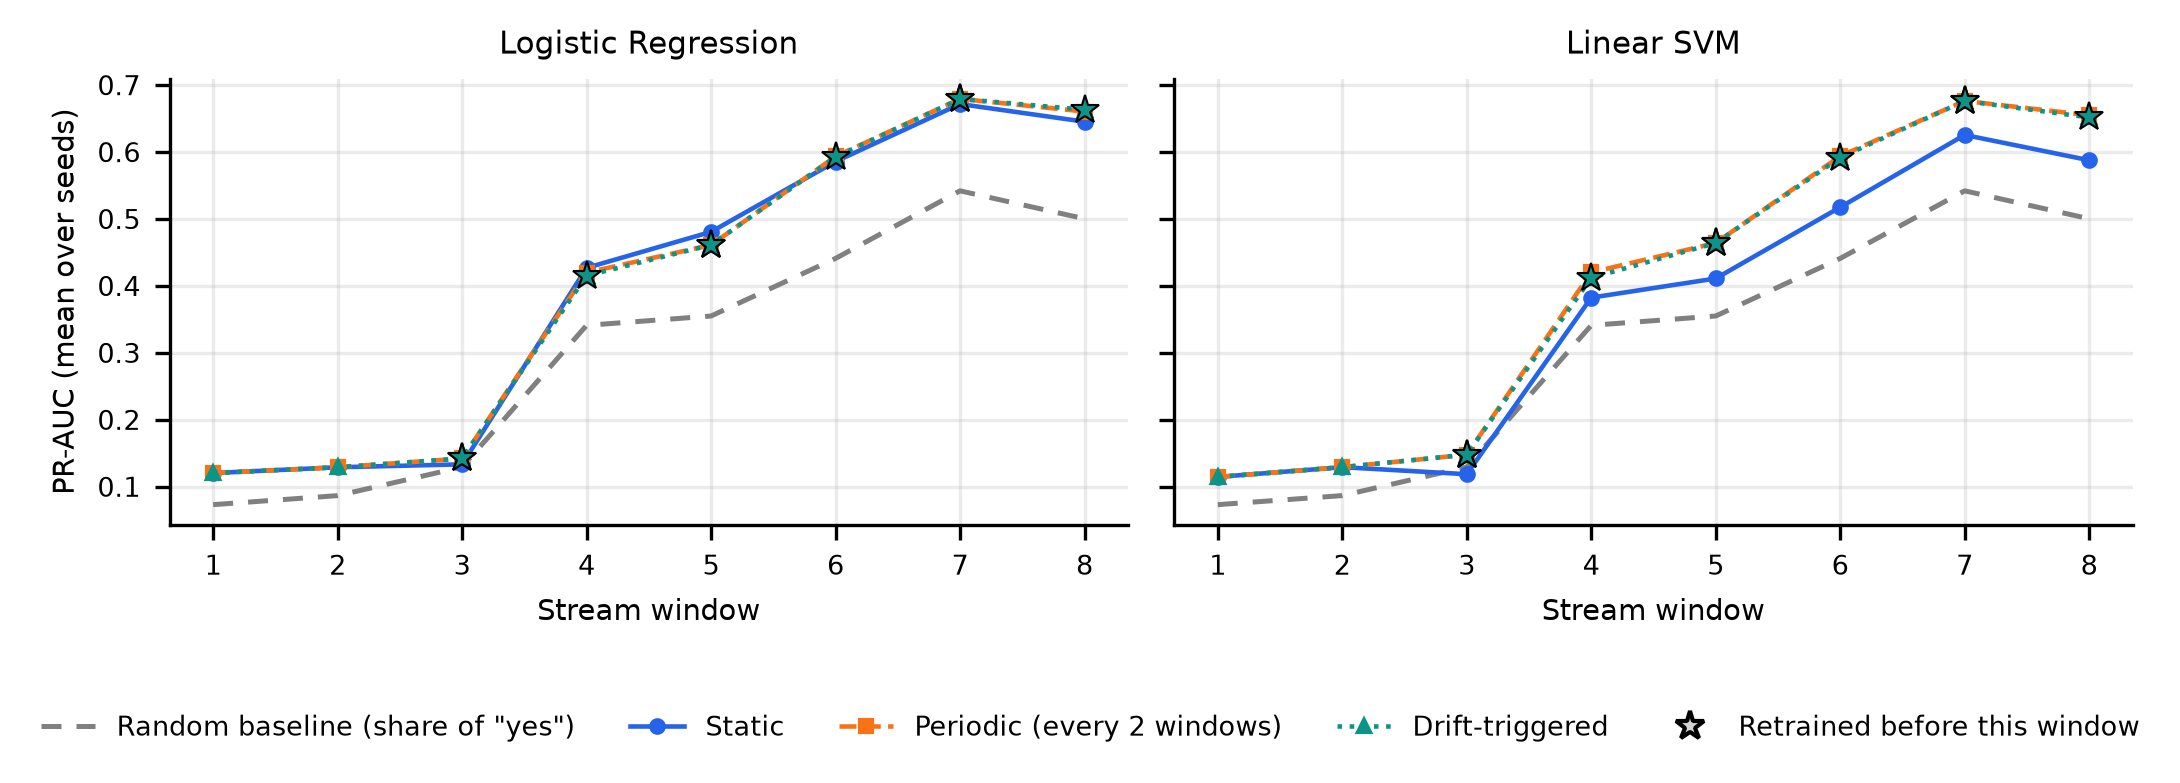
\includegraphics[width=\textwidth]{figures/14_real_replay_pr_auc.png}
\caption{Real replay: PR-AUC per window for the three strategies with each window's random baseline. Raw PR-AUC rises alongside the share of ``yes'' (the random baseline).}
\label{fig:realpr}
\end{figure*}

\begin{figure*}[t]
\centering
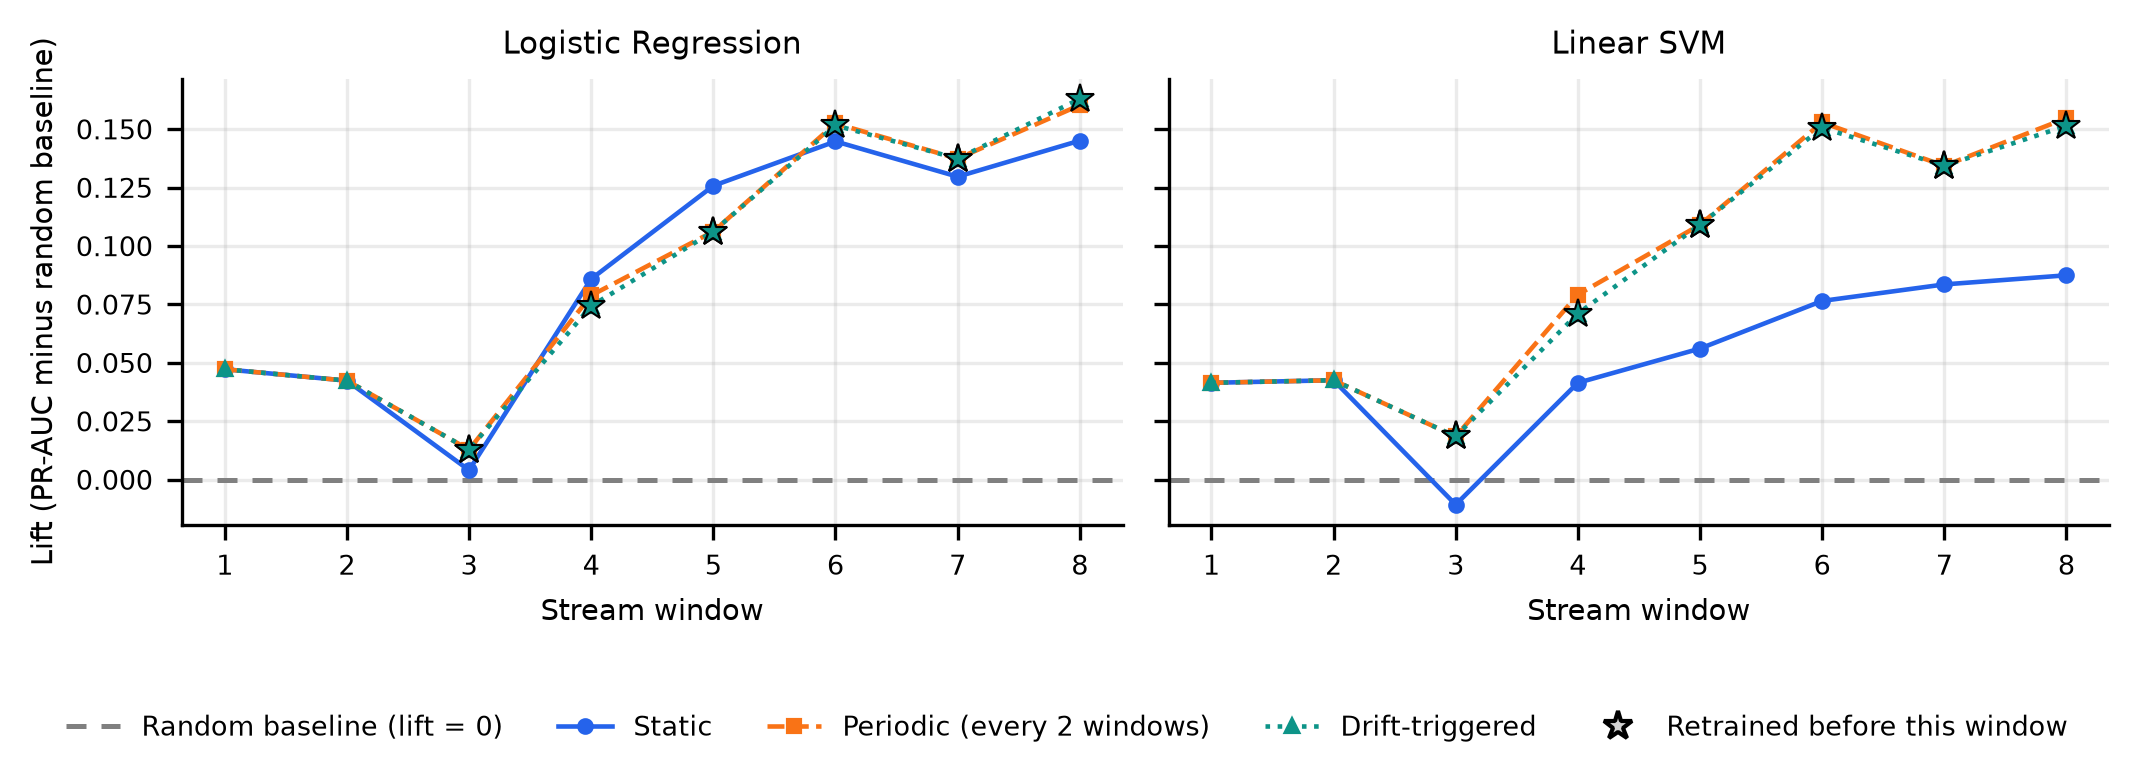
\includegraphics[width=\textwidth]{figures/16_real_replay_lift.png}
\caption{Real replay: lift (PR-AUC minus random baseline) per window. The strategies overlap for Logistic Regression.}
\label{fig:reallift}
\end{figure*}

Drift-triggered retraining did not beat periodic retraining; it retrained six times against three, at roughly twice the retraining time, for the same PR-AUC. After retraining, recall rose (0.511 to 0.639 for Logistic Regression) and precision fell (0.359 to 0.323) while F1 barely changed, which is consistent with the re-tuned threshold trading precision for recall rather than with better ranking.

\subsection{Synthetic scenarios}

In all three corrected synthetic scenarios the strategies are within about 0.002 PR-AUC of each other (Fig.~\ref{fig:synth}). For Logistic Regression, mean PR-AUC was 0.057/0.058/0.057 (static/periodic/drift-triggered) in the stationary scenario (random 0.047), 0.052/0.052/0.052 in the sudden scenario (random 0.045) and 0.052/0.054/0.053 in the gradual scenario (random 0.045); Linear SVM was similar. Models in these scenarios are close to random (lift at most 0.010), which may be because the synthetic pools come from the early training period, where the model has little signal (not tested).

\begin{figure*}[t]
\centering
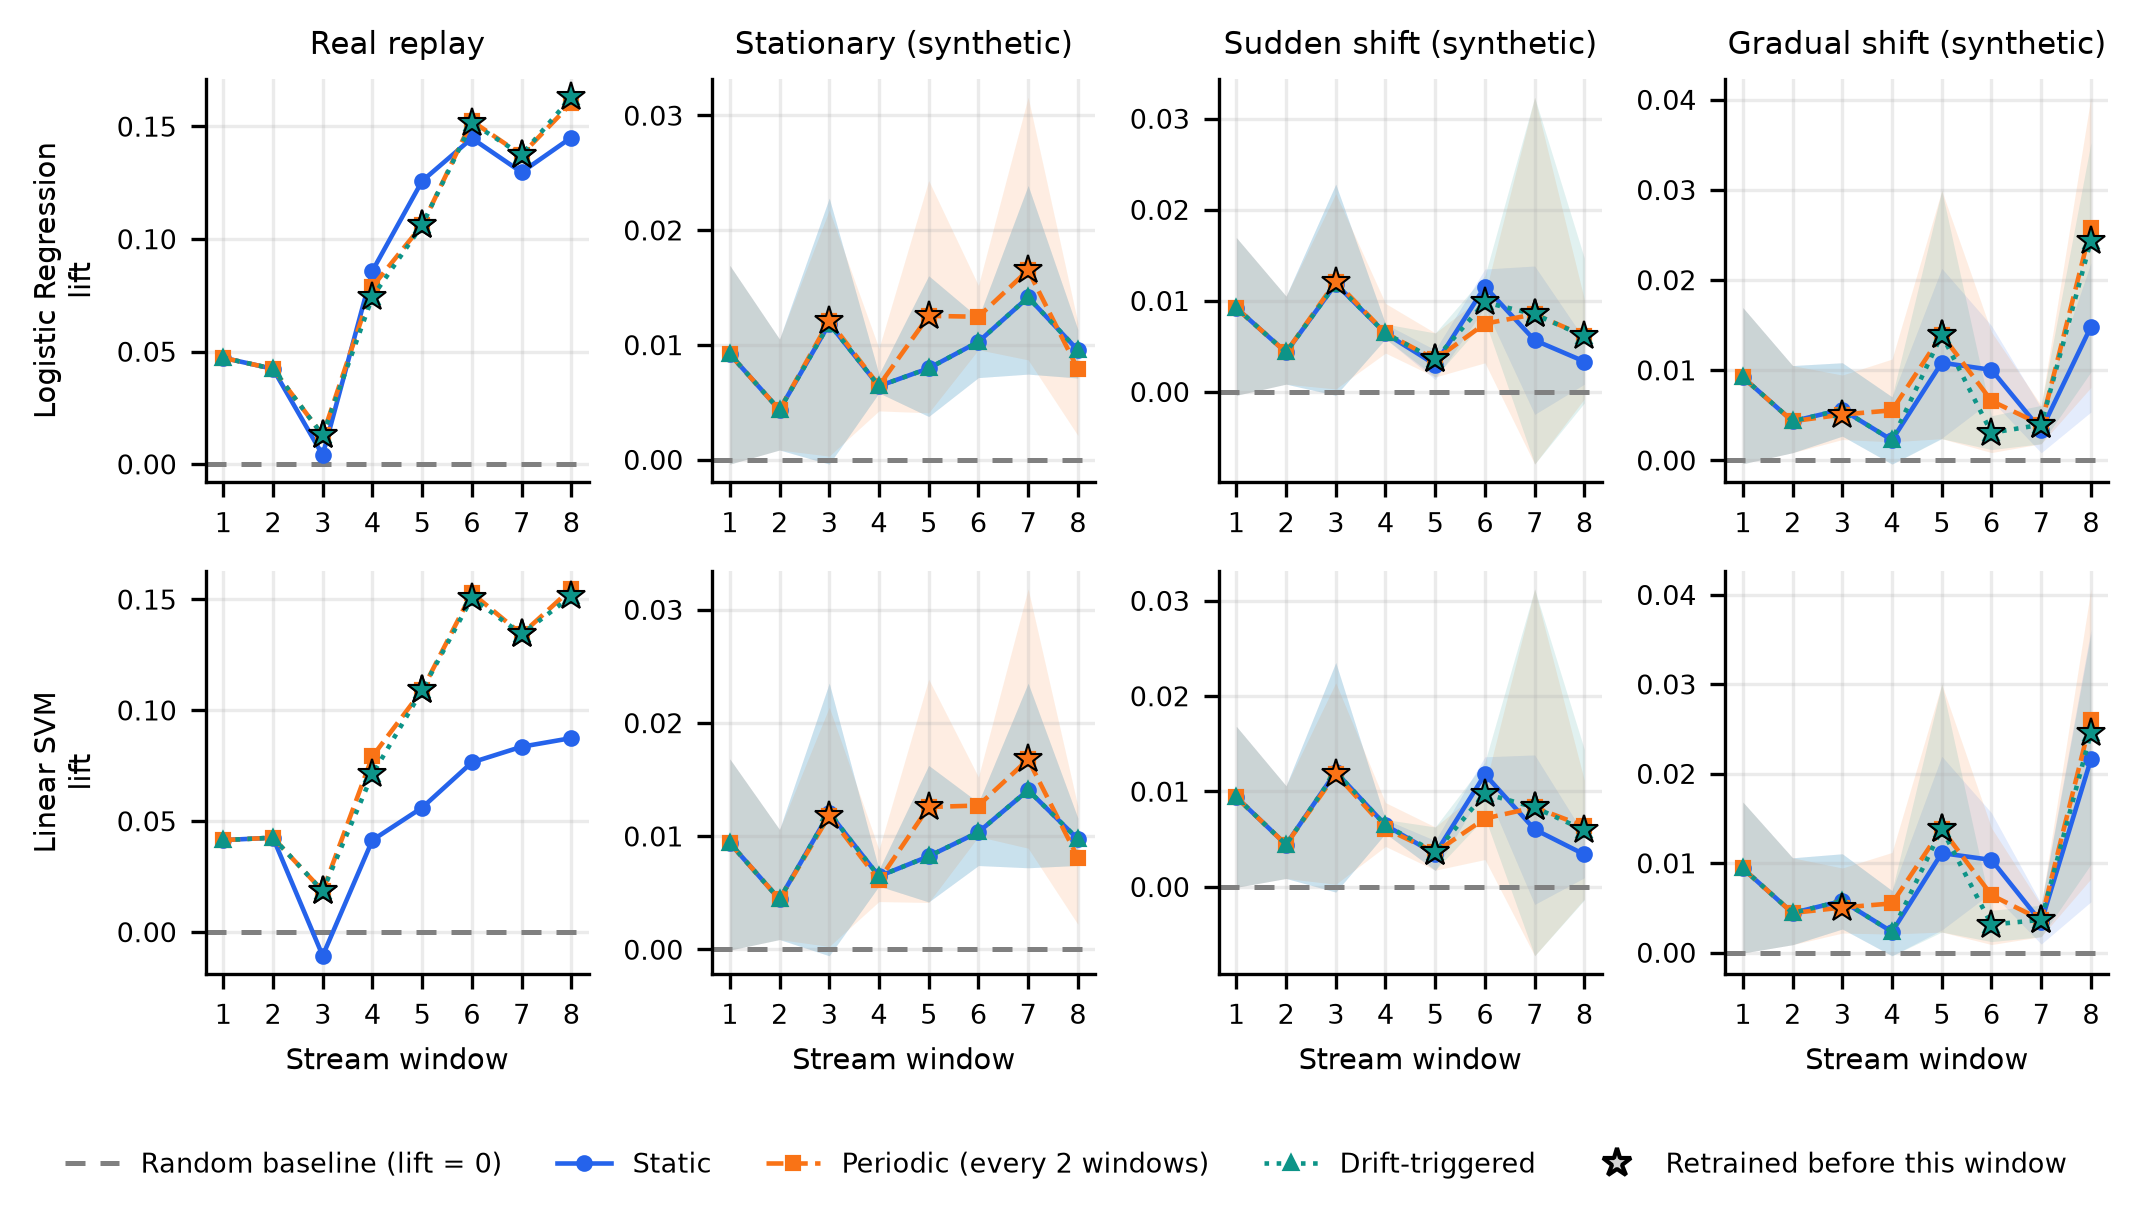
\includegraphics[width=\textwidth]{figures/17_all_scenarios_lift.png}
\caption{Lift per window for all scenarios, strategies and models (corrected synthetic design). In synthetic scenarios all strategies stay close to the random baseline.}
\label{fig:synth}
\end{figure*}

\subsection{Drift detection}

Table~\ref{tab:detect} reports alarm behavior, measured on the static strategy's rows so that the reference stays fixed. In the synthetic scenarios the alarm worked as designed: no false alarms in any seed, a delay of 0 windows for the sudden shift and 2 windows for the gradual shift. In the real replay, however, the alarm fired in all 8 windows, starting with window 1 (Fig.~\ref{fig:alerts}). The model inputs that moved most were \texttt{previous} and \texttt{poutcome} (PSI 1.1--4.0), consistent with later rows containing many more repeat customers (Fig.~\ref{fig:realdrift}). Since the reference after a retrain is the expanding history, still dominated by old rows, the alarm keeps firing, and drift-triggered retraining becomes ``retrain whenever new labels arrive''.

\begin{table}[t]
\caption{Drift alarm behavior (all 3 seeds identical)}
\label{tab:detect}
\centering
\footnotesize
\begin{tabular}{@{}lccc@{}}
\toprule
Scenario & Alerts & False alarms & Delay \\
\midrule
Real replay & 8 of 8 & -- & none known \\
Stationary & 0 of 8 & 0 & -- \\
Sudden (change at 5) & 4 of 8 & 0 & 0 windows \\
Gradual (change from 3) & 4 of 8 & 0 & 2 windows \\
\bottomrule
\end{tabular}
\end{table}

\begin{figure*}[t]
\centering
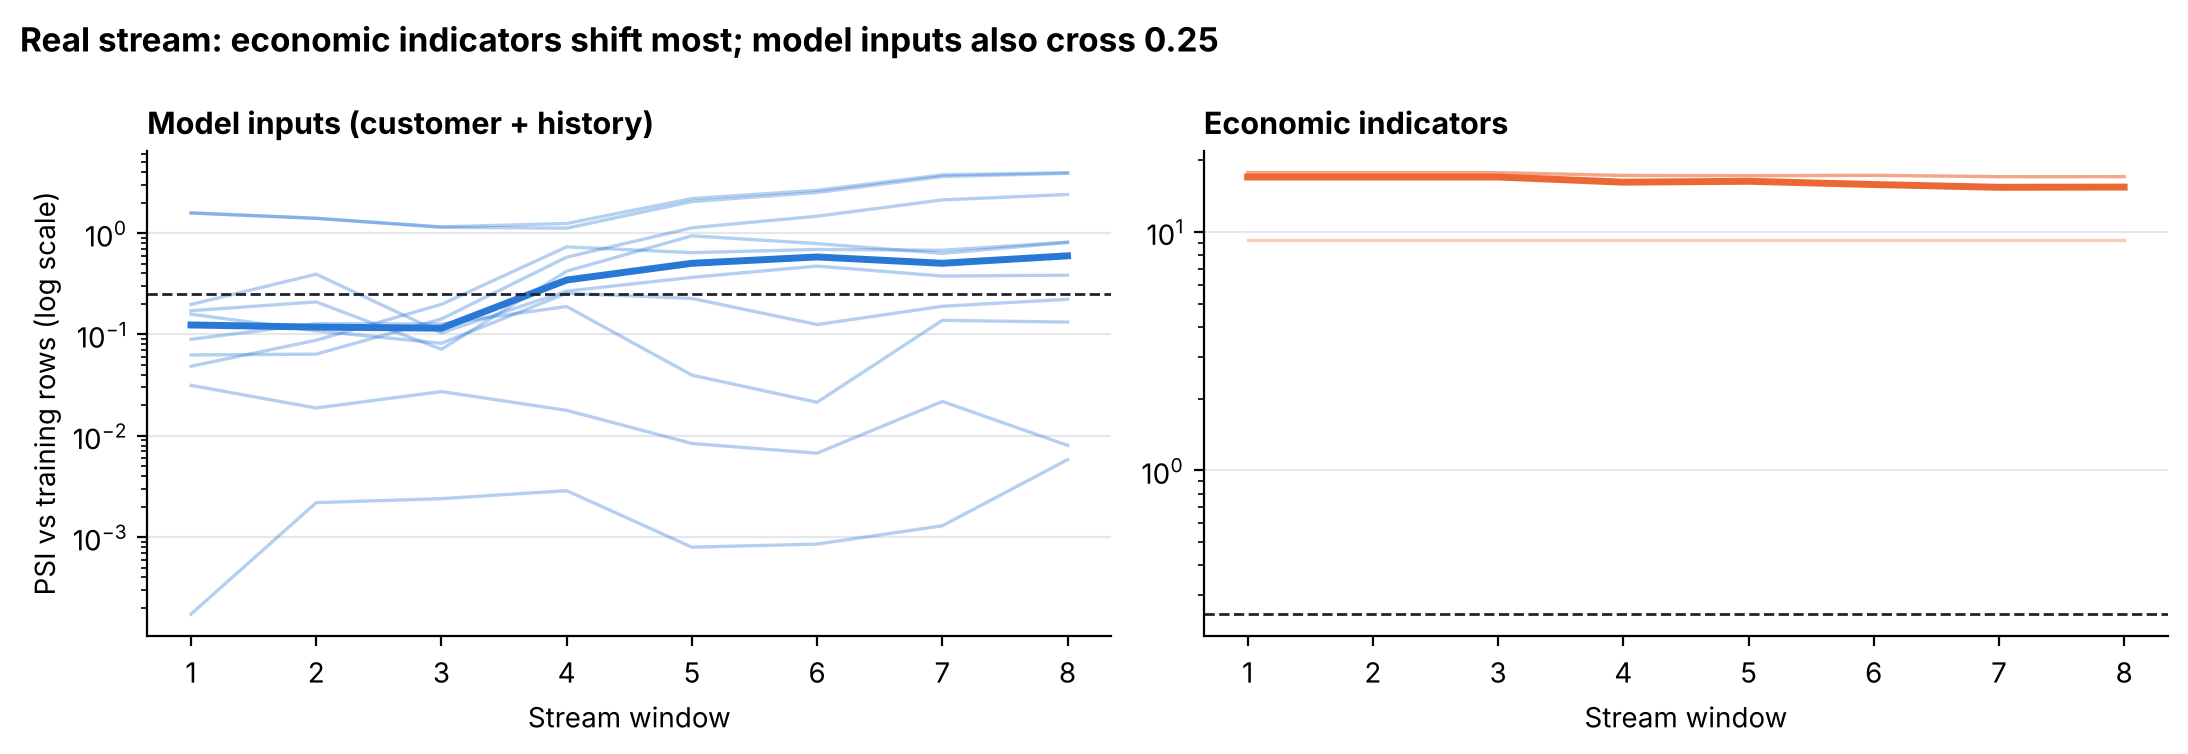
\includegraphics[width=\textwidth]{figures/12_real_replay_drift_by_group.png}
\caption{Real replay: PSI of each feature against the training rows (log scale; dashed line = 0.25 alert threshold). At least one model input exceeds 0.25 in every window, and every economic indicator exceeds it by a wide margin.}
\label{fig:realdrift}
\end{figure*}

\begin{figure*}[t]
\centering
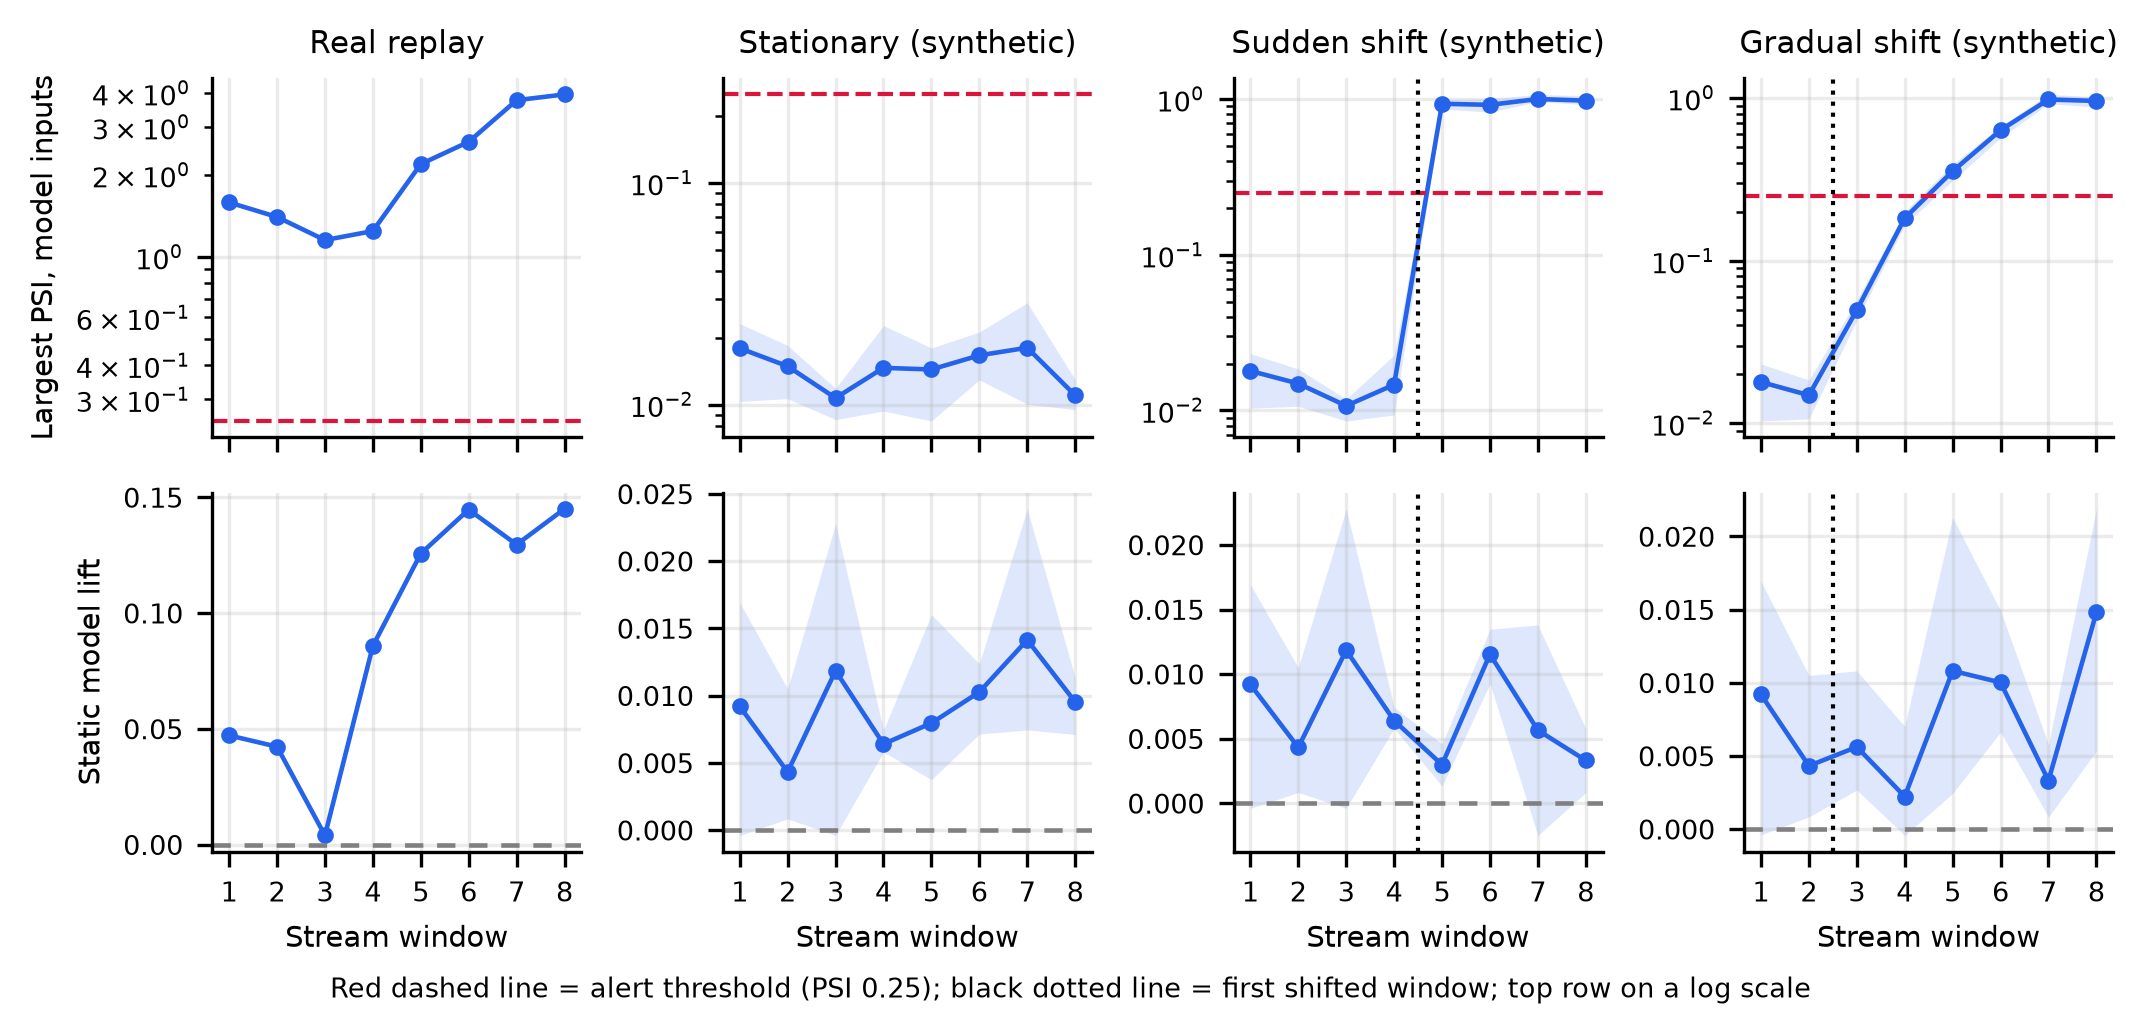
\includegraphics[width=\textwidth]{figures/18_alerts_vs_static_performance.png}
\caption{Drift alerts (fixed reference) against the static model's performance. Alerts in the real replay fire in every window; in synthetic scenarios they correctly mark the change, but the static model's lift does not drop afterward.}
\label{fig:alerts}
\end{figure*}

\subsection{Uncertainty and cost}

The paired bootstrap (Fig.~\ref{fig:boot}) confirms the picture. For real-replay Logistic Regression, periodic minus static is $+0.0016$ (95\% interval $-0.0066$ to $+0.0108$) and drift-triggered minus static is $+0.0013$ ($-0.0073$ to $+0.0102$); both include zero. For Linear SVM the gains are $+0.0393$ ($+0.0266$ to $+0.0522$) and $+0.0376$ ($+0.0249$ to $+0.0506$). These intervals reflect within-window sampling variation only (not independent replications or temporal dependence), the real replay is a single deterministic run, and the static SVM started weaker, so this result does not establish a general retraining advantage. In every synthetic scenario every interval includes zero (for drift-triggered minus static in the stationary scenario the difference is exactly zero, because that strategy never retrained).

No single retrain took longer than about 1.04~s. Drift monitoring cost on average about 1.3--1.4~s per real-replay run, a cost only the drift-triggered strategy needs. In absolute terms all costs were small, but drift-triggered retraining paid both the monitoring cost and twice the retraining cost of periodic retraining, for no additional PR-AUC.

\begin{figure*}[t]
\centering
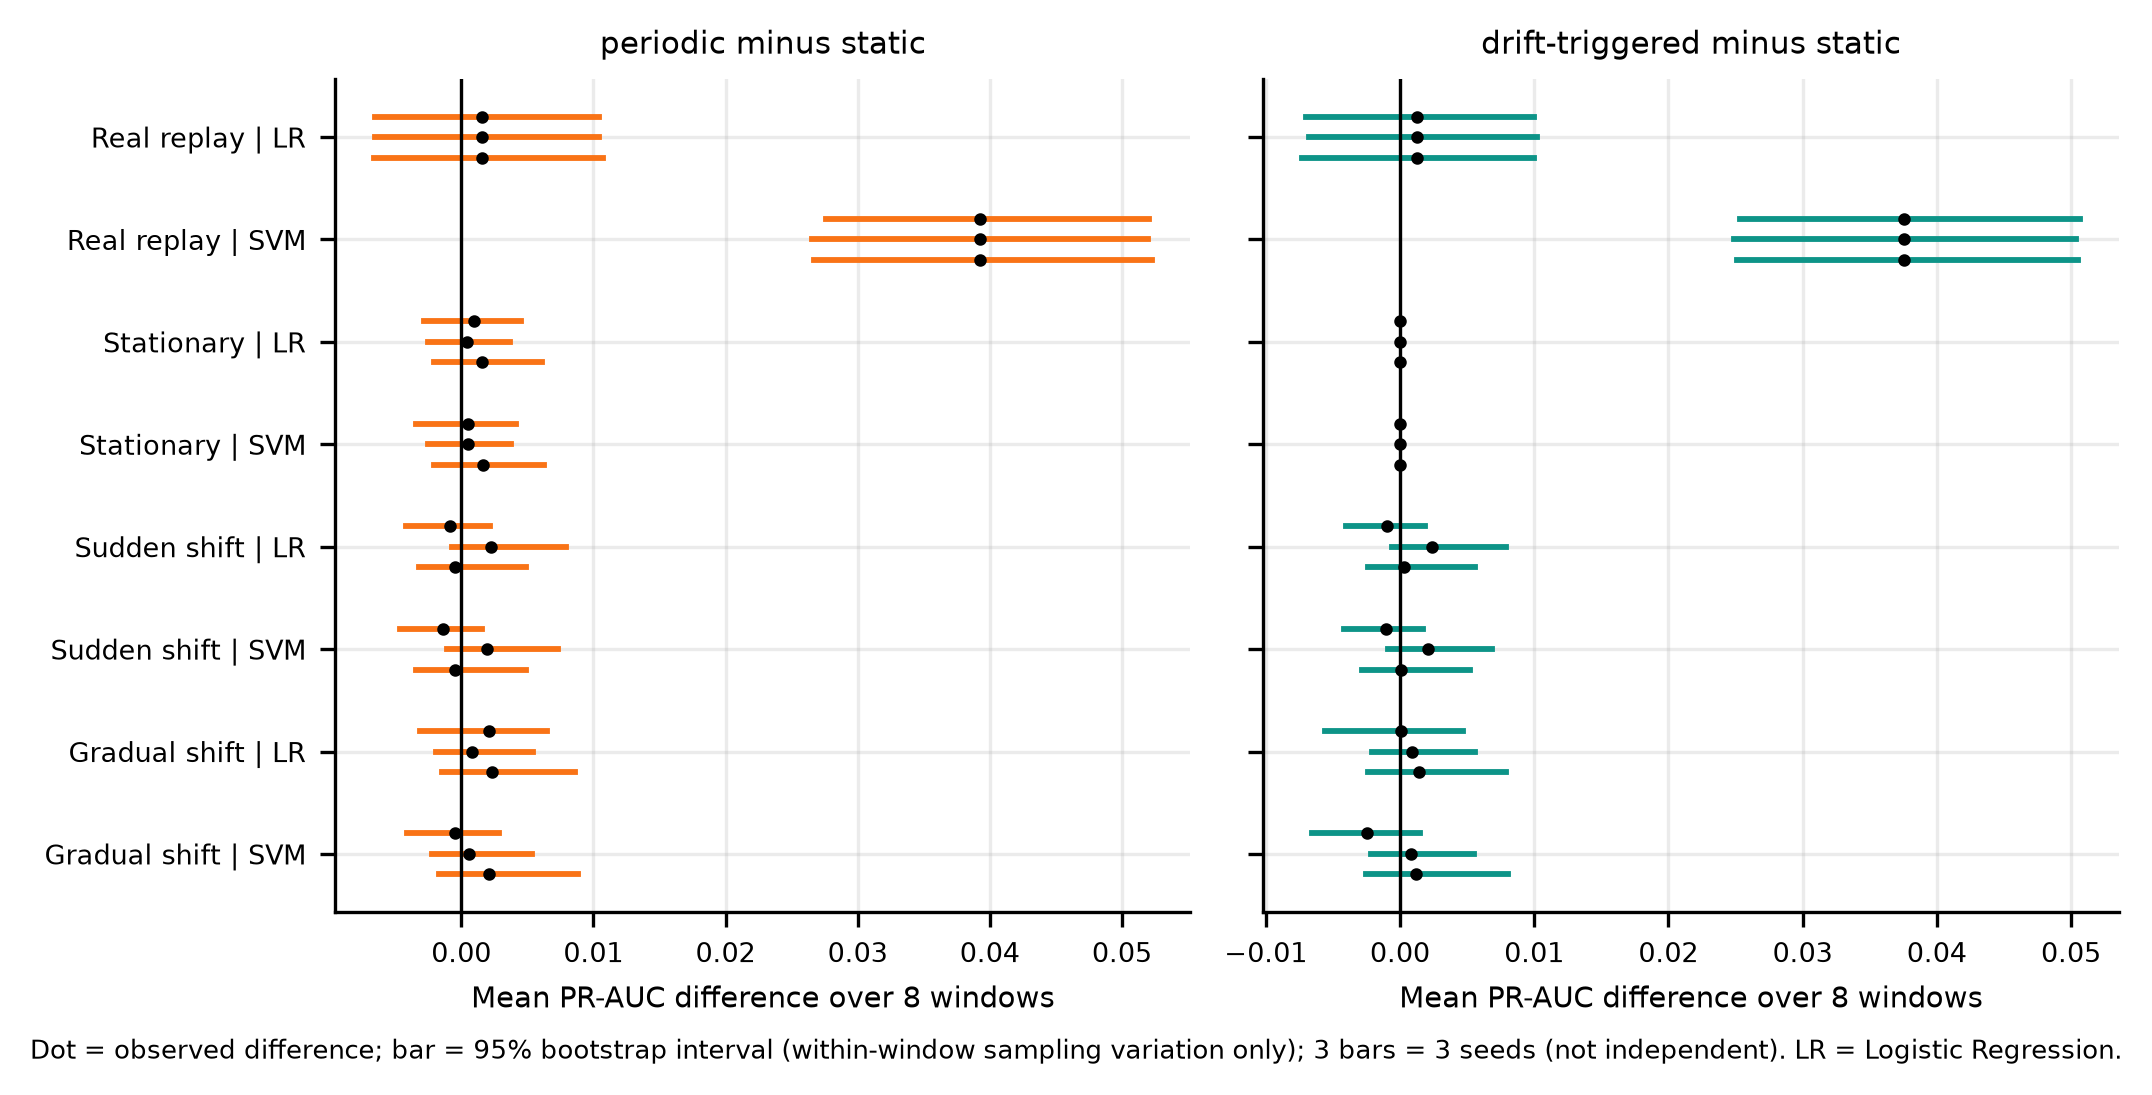
\includegraphics[width=\textwidth]{figures/21_bootstrap_intervals.png}
\caption{Paired bootstrap 95\% intervals for the mean PR-AUC difference versus static. Only the real-replay Linear SVM excludes zero. Intervals reflect within-window sampling variation only.}
\label{fig:boot}
\end{figure*}

%======================================================================
\section{Discussion}
\label{sec:discussion}

\subsection{Why the strategies performed alike}

\textbf{Weak signal and a moving baseline.} In the real replay the share of ``yes'' rises from 7.3\% in window 1 to 54.2\% in window 7, and static PR-AUC rises from 0.120 to 0.671. About 85\% of that rise (0.469 of 0.551) corresponds numerically to the rise in the random-ranking baseline, which for PR-AUC equals the share of ``yes'' by definition; the lift changed much less (0.047 to 0.130) (Fig.~\ref{fig:yes}). This is a descriptive comparison, not a causal decomposition, and not a claim about customers or the economy; it is why we report lift. In window 3 the static model's ROC-AUC (0.479) was even below 0.5.

\begin{figure*}[t]
\centering
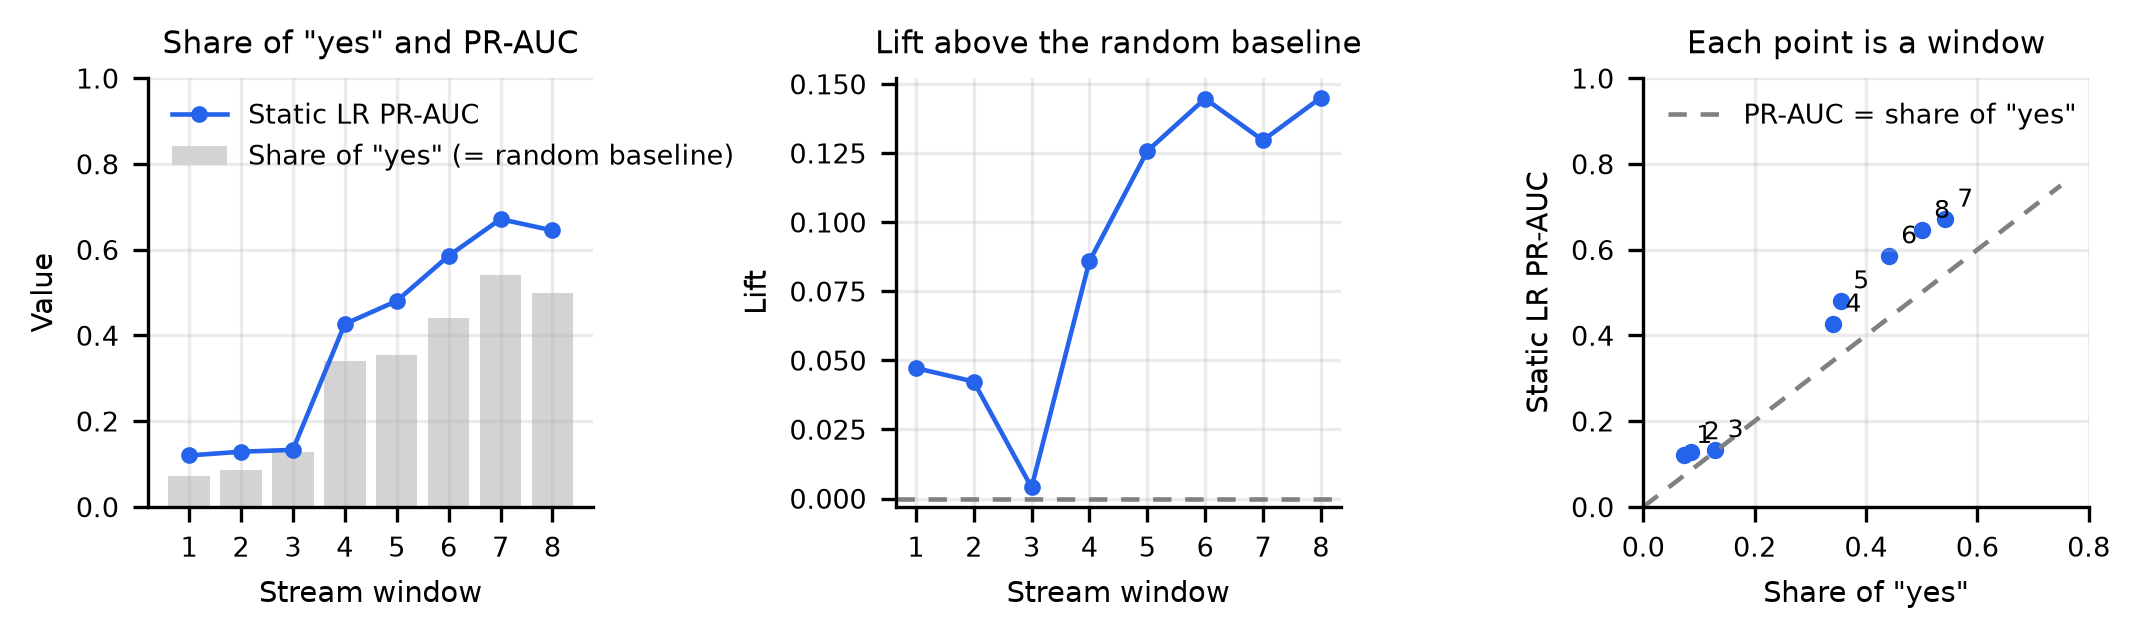
\includegraphics[width=\textwidth]{figures/19_real_replay_yes_share_vs_pr_auc.png}
\caption{Real replay: share of ``yes'', static PR-AUC and lift per window. Most of the rise in raw PR-AUC corresponds numerically to the rise in the random baseline.}
\label{fig:yes}
\end{figure*}

\textbf{Previous-campaign success and the model's recall.} The error analysis of static Logistic Regression (Fig.~\ref{fig:error}) shows that it caught 99.5\% of subscribers whose previous campaign succeeded (827 of 831), but only 22.3\% after a previous failure and 45.5\% with no previous contact. Of the 1,047 subscribers it missed, 1,043 had no successful previous campaign. Our subgroup analysis suggests that previous-campaign success is strongly associated with the model's ability to identify subscribers. However, this descriptive analysis does not establish that other features contribute no predictive information.

\begin{figure*}[t]
\centering
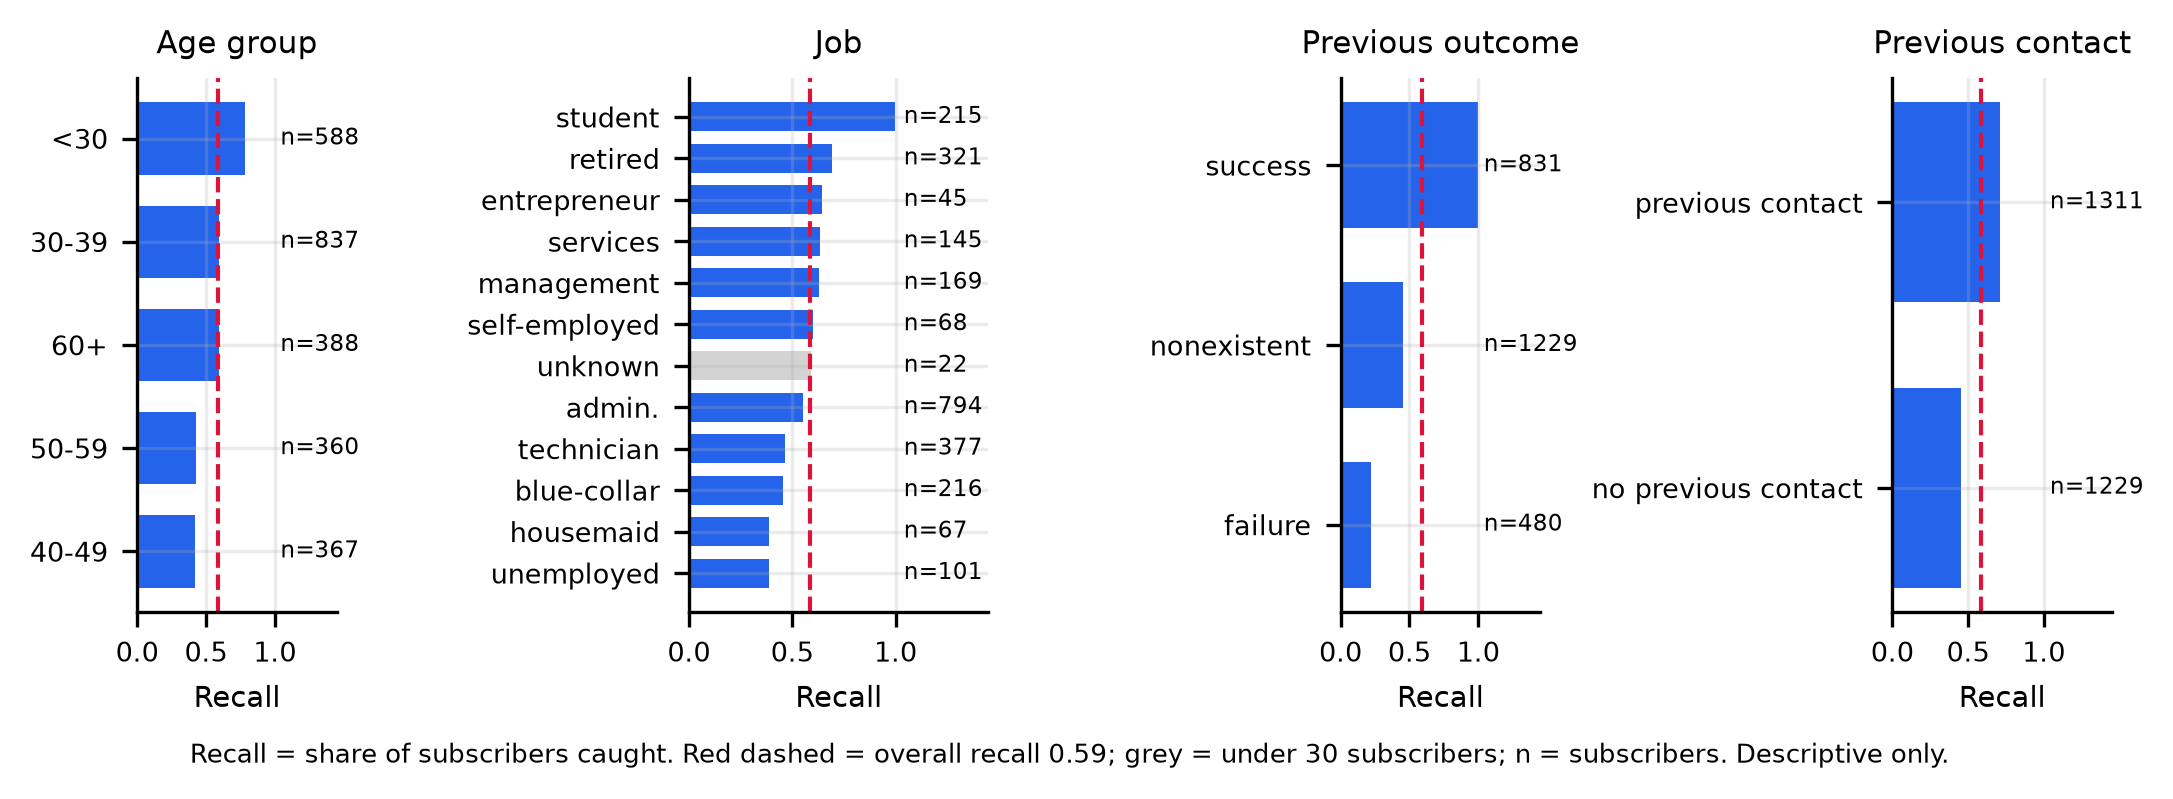
\includegraphics[width=\textwidth]{figures/22_error_analysis_recall_by_group.png}
\caption{Error analysis (real replay, static Logistic Regression): recall by age group, job, previous outcome and previous contact. Descriptive only; not a measure of feature importance.}
\label{fig:error}
\end{figure*}

\textbf{Retraining changes the training data only a little.} With an expanding history, even after six retrains only 20.0\% of the drift-triggered model's training rows come from the stream (6,178 of 30,890; Fig.~\ref{fig:comp}). The original rows, with 4.8\% ``yes'', dominate.

\begin{figure*}[t]
\centering
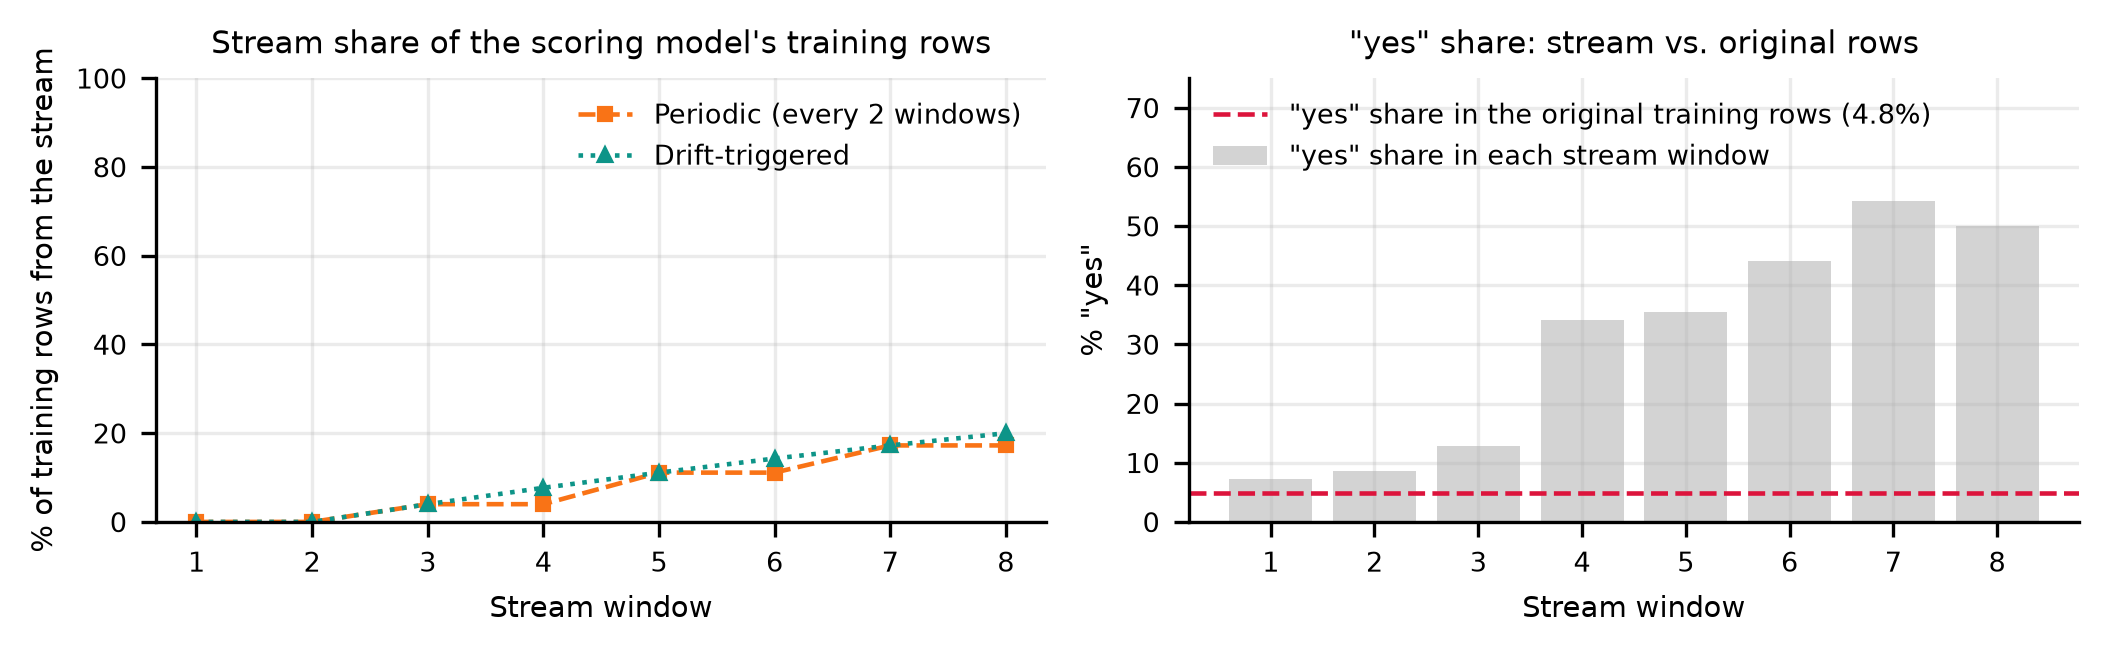
\includegraphics[width=\textwidth]{figures/23_real_replay_training_set_composition.png}
\caption{Real replay, Logistic Regression, seed 42. Left: share of the scoring model's training rows that come from the stream, for periodic and drift-triggered retraining; old rows dominate the expanding history. Right: share of ``yes'' in each stream window compared with the original training rows (4.8\%).}
\label{fig:comp}
\end{figure*}

\textbf{Within-window cross-validation: the two models differ.} For Logistic Regression the diagnostic averaged 0.407, below the static model's 0.417 on the same held-out rows (Fig.~\ref{fig:cv}), which gives no sign that a lack of recent labels limits it at this sample size. For Linear SVM it averaged 0.405, above the static model's 0.377, which is consistent with retraining helping the weaker SVM. The diagnostic uses labels that would not be available at prediction time and trains each fold on about 30 times fewer rows than the static model, so it is a small-sample diagnostic, not a performance ceiling, and it cannot rule out gains from more recent data at larger sample sizes.

\begin{figure*}[t]
\centering
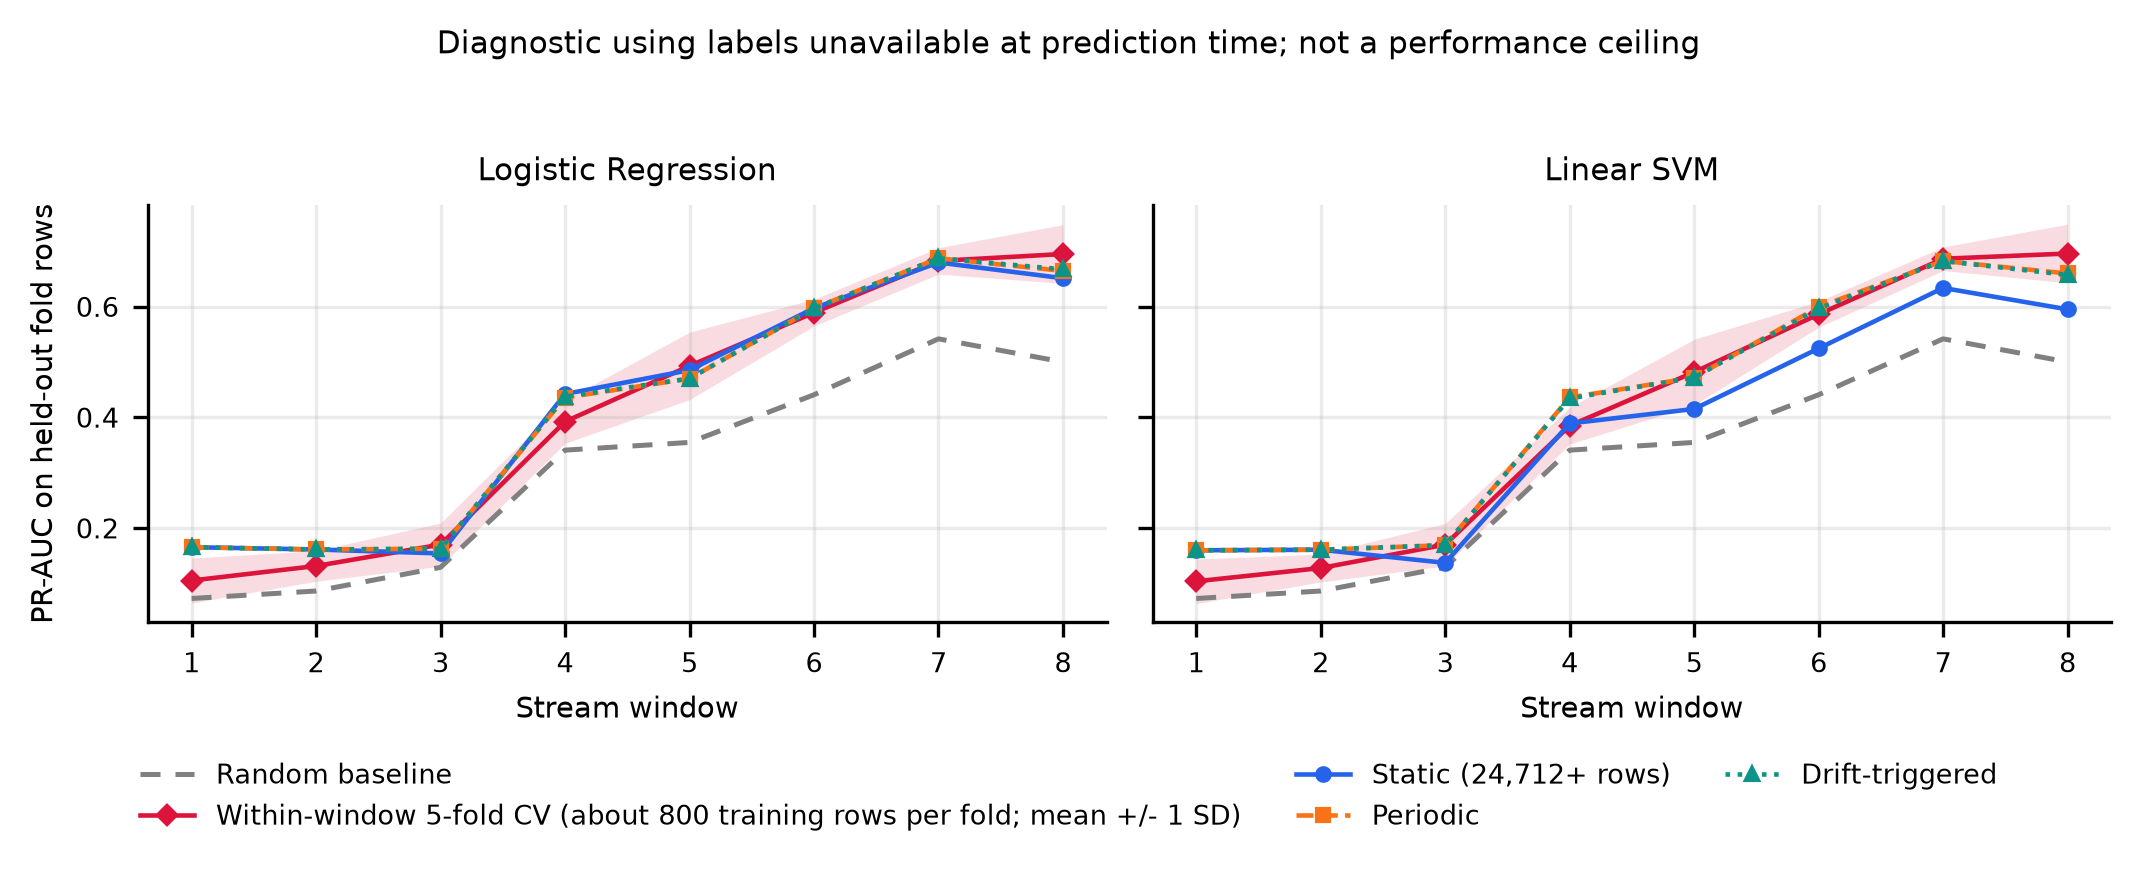
\includegraphics[width=\textwidth]{figures/20_oracle_ceiling.png}
\caption{Within-window 5-fold cross-validation diagnostic (about 800 training rows per fold) against the three strategies. A small-sample diagnostic, not a performance ceiling.}
\label{fig:cv}
\end{figure*}

\textbf{Detected drift was not shown to hurt the model.} We keep three things apart: an observed distribution shift (PSI), a drop in predictive performance, and a demonstrated benefit from retraining. In the synthetic scenarios the age shift was detected promptly (PSI 0.83--1.07 after the sudden change), yet the static model's lift did not measurably drop after the change (mean change $-0.0021$ sudden, $+0.0010$ gradual, with mixed signs across seeds), and the models there are close to random, so there was little to lose. In the real replay the alarm fired in every window, so we cannot link the shift to any performance drop. We did not test for concept drift, and nothing here establishes it. This was the most important lesson for us: \emph{detecting a change in the data does not mean the model's performance has deteriorated, or that retraining will help.}

\subsection{Responding to TA feedback}

\textbf{(1) Tune the threshold; show subscribers found and wrong ``yes'' predictions.} The midterm baseline predicted zero ``yes'' at a fixed 0.5 threshold. Thresholds are now tuned for best F1, on development rows for model selection and on the most recent labeled rows at every fit in the stream, and confusion counts are reported (Section~\ref{sec:models}, Table~\ref{tab:confusion}).

\textbf{(2) Show whether drift alerts actually help.} They did not help in our setting. Real-replay alerts fired in every window and so could not separate windows; synthetic alerts were correct but did not coincide with performance drops; and drift-triggered retraining matched periodic retraining at twice the number of retrains.

\textbf{(3) Fair comparison.} All strategies share one loop, stream, model, feature set, seed set and threshold rule, and a unit test verifies they are identical before the first retrain.

\subsection{What correcting our own flaw taught us}

Under the original synthetic design, retraining appeared to help: for Logistic Regression, periodic minus static was $+0.0054$ (sudden) and $+0.0040$ (gradual). After the correction these fell to $+0.0003$ and $+0.0017$ (Table~\ref{tab:v1v2}).

\begin{table}[t]
\caption{Retraining gain over static before (v1) and after (v2) the row-reuse correction (Logistic Regression, mean PR-AUC difference)}
\label{tab:v1v2}
\centering
\footnotesize
\begin{tabular}{@{}lcccc@{}}
\toprule
 & \multicolumn{2}{c}{Periodic $-$ static} & \multicolumn{2}{c}{Drift $-$ static} \\
Scenario & v1 & v2 & v1 & v2 \\
\midrule
Stationary & $+0.0020$ & $+0.0010$ & $0.0000$ & $0.0000$ \\
Sudden & $+0.0054$ & $+0.0003$ & $+0.0062$ & $+0.0006$ \\
Gradual & $+0.0040$ & $+0.0017$ & $+0.0042$ & $+0.0008$ \\
\bottomrule
\end{tabular}
\end{table} The two designs differ in more than one factor (v2 also fits the initial model on 60\% rather than 80\% of the training rows and uses different draws), so this comparison does not isolate row reuse as the only cause, but it is consistent with reuse having inflated the earlier result. Catching this changed our conclusions, and we now consider leakage checks between retraining and evaluation data an essential part of any retraining study.

%======================================================================
\section{Deployment and Complexity}
\label{sec:deployment}

\textbf{Deployment.} A bank could run this system as a batch process before each campaign: (1) score customers on the planned call list with the current model and threshold; (2) record outcomes as calls are made; (3) after the label delay, add labeled outcomes to the training history; (4) retrain on a fixed schedule, which our results suggest is as effective as drift-triggered retraining here; and (5) compute PSI per feature each period and log alerts for human review, rather than retraining automatically on every alert. Monitoring could weight features by their importance to the model (not tested here), because in our synthetic scenarios a detected input shift did not coincide with a performance drop.

\textbf{Complexity.} Let $n$ be the number of training rows and $d = 40$ the number of encoded columns. Fitting Logistic Regression or a linear SVM costs roughly $O(n\,d)$ per iteration of the optimizer; with an expanding history, $n$ grows by one window per retrain, so retraining cost grows linearly with time. Computing PSI for one feature requires quantiles of the reference sample ($O(n \log n)$ to sort, reusable across windows) and $O(m)$ to bin a window of $m$ rows; monitoring 15 features is therefore linear in the window size. In practice, no retrain took longer than about 1.04~s on about 25,000--31,000 rows, and monitoring took about 0.2~s per window. At much larger scale, a sliding training window would cap $n$, and the quantile edges can be cached.

\textbf{Reproducibility.} Our final analyses (notebooks 06b and 07 and the unit tests) were run in Python~3.12 with pinned package versions (pandas~3.1.0, NumPy~2.5.4, scikit-learn~1.9.1, SciPy~1.18.1, Matplotlib~3.11.2); notebooks 04--06 were executed in separate Python~3.13 environments, and we did not repeat a clean-environment run of the full pipeline. Shared settings (split fractions, feature lists, seeds and drift thresholds) are defined once in a settings module and imported everywhere. The README documents how to download the dataset and verify its SHA-256 checksum. The notebooks are numbered in run order.
A suite of 67 unit tests checks the rules the results depend on, including row order, the exclusion of \texttt{duration}, label delay and the absence of overlap between scored and training rows. Both the original and the corrected experiment outputs are kept, so the correction in Section~\ref{sec:drift} can be audited.

%======================================================================
\section{Project Journey and Team Process}
\label{sec:journey}

\textbf{How we split the work.} After the midterm, where the team jointly built the exploratory analysis, leakage review, chronological split and first baseline, we divided the final phase into four independent parts, each on its own Git branch with a pull request (Table~\ref{tab:team}). Each part had a clear handoff: drift detection and scenarios feed the strategy loop, model selection feeds the shortlist used in the loop, and the loop's results file feeds the analysis.

\begin{table}[t]
\caption{Division of work in the final phase}
\label{tab:team}
\centering
\footnotesize
\begin{tabular}{@{}p{1.9cm}p{5.9cm}@{}}
\toprule
Member & Responsibility \\
\midrule
Rutuja Saste & Drift detection (PSI, KS, trigger rule) and the four scenarios \\
Tanya Shah & Model comparison, threshold tuning, economic-feature test, final slides \\
Himja Patel & Retraining strategies, shared experiment loop and full run \\
Uday Patel & Results analysis, row-reuse correction, report and repository \\
\bottomrule
\end{tabular}
\end{table}

\textbf{How we coordinated.} We coordinated through WhatsApp and a shared work plan that listed each person's deliverables and the default settings everyone would start from. Every consequential choice, such as the prediction moment, the split, the feature set and the drift threshold, was recorded in a decision log in the repository, with proposed defaults kept separate from confirmed decisions. Unit tests (67 by the end) guarded the rules that mattered most: no shuffling, no use of \texttt{duration}, no future labels in retraining and no overlap between scored and training rows.

\textbf{What we expected and what surprised us.} We began expecting drift detection to make retraining more efficient: instead of retraining on a schedule, we would retrain only when needed and keep similar or better performance with fewer retraining events. That is not what happened. In the real replay, drift-triggered retraining ran six times against three for periodic retraining without a clear improvement, and some of the gains we first saw in synthetic experiments came from repeated records appearing in both retraining and evaluation data. These surprises changed how we think about the problem. We started out asking whether drift detection could make retraining more efficient; we finished understanding that a change in the data is not the same as a decline in the model, and that a retraining policy is only as useful as the signal the model has to learn from.

%======================================================================
\section{Use of AI Tools}
\label{sec:ai}

We used AI assistants during this project and disclose how. Anthropic's Claude Code was used as a coding assistant under written project rules (an \texttt{AGENTS.md} file): it worked one approved step at a time, explained each change, never staged or committed code (only students made Git commits), never invented results, and recorded decisions and explanations in the decision log and a learning log. Claude was also used as a tutor to explain methods, to review our code and results critically, and to help draft and edit this report. An AI-assisted review first flagged the possible row-reuse problem described in Section~\ref{sec:drift}; we then measured the overlap ourselves before correcting it. All design decisions were made by the team, every number in this report was checked against our notebooks and saved results, and all team members reviewed the draft. % TEAM: each member should confirm which AI tools they used for their own part and edit this paragraph if needed.

%======================================================================
\section{Limitations and Future Work}

Our real-data evidence comes from one deterministic stream of 8 windows; its three seeds are identical, and the synthetic seeds resample one fixed set of rows, so neither provides independent replications. Bootstrap intervals reflect within-window sampling only. The models are weak (real-replay lift about 0.09), which limits how much any strategy can recover. The drift rule was not selective in the real replay, so we could not test whether a selective trigger would help. All stream settings (8 windows, one-window label delay, retraining every two windows, PSI~$>$~0.25, expanding history) were proposed before the experiment and not tuned on it; because the team has now seen the stream results, any changed setting must be reported as a secondary analysis. The synthetic scenarios rest on assumption A6, and threshold-based metrics depend on re-tuned cut-offs. We did not test for concept drift; the input shifts and the rising share of ``yes'' are descriptive and do not show that the relationship between inputs and outcome changed.

Natural next steps follow from these findings: (1) a sliding or recency-weighted training window, so retraining reflects recent data; (2) a drift rule that compares each window with the previous one, or weights features by their importance, so alarms fire only on changes that matter; (3) selecting such settings on a replay of the development period, then running them once on the stream; and (4) testing whether the current-contact features, once their availability is established, add enough signal for retraining strategies to differ.

%======================================================================
\section{Conclusion}

We asked whether drift-triggered retraining keeps a classical model's predictions better than static or periodic retraining. On our single real bank-marketing stream it did not: the three strategies performed alike for Logistic Regression, retraining helped only a weaker Linear SVM reach about the same level, and drift-triggered retraining doubled the retraining work without additional benefit. Our diagnostics are consistent with weak predictive signal, rather than model staleness, being the main limitation: previous-campaign success is strongly associated with the model's recall, alarms on detected input shifts did not coincide with performance drops, and a small-sample within-window cross-validation diagnostic did not beat the static Logistic Regression (although it exceeded the static Linear SVM). For practitioners, the lesson is to measure whether drift hurts the model before retraining automatically.

\section*{Acknowledgment}
We thank Prof.\ Shih Yu Chang for guidance throughout DATA~245 and our teaching assistant, Sooror, for feedback on the midterm presentation that shaped the final experiment. Code, notebooks and results are available at \url{https://github.com/UdayPate/ML-drift-project}.

\begin{thebibliography}{10}

\bibitem{gama2014survey}
J.~Gama, I.~\v{Z}liobait\.{e}, A.~Bifet, M.~Pechenizkiy, and A.~Bouchachia, ``A survey on concept drift adaptation,'' \emph{ACM Computing Surveys}, vol.~46, no.~4, art.~44, 2014.

\bibitem{lu2019review}
J.~Lu, A.~Liu, F.~Dong, F.~Gu, J.~Gama, and G.~Zhang, ``Learning under concept drift: A review,'' \emph{IEEE Trans.\ Knowledge and Data Engineering}, vol.~31, no.~12, pp.~2346--2363, 2019.

\bibitem{webb2016characterizing}
G.~I.~Webb, R.~Hyde, H.~Cao, H.~L.~Nguyen, and F.~Petitjean, ``Characterizing concept drift,'' \emph{Data Mining and Knowledge Discovery}, vol.~30, no.~4, pp.~964--994, 2016.

\bibitem{massey1951ks}
F.~J.~Massey, ``The Kolmogorov--Smirnov test for goodness of fit,'' \emph{J.\ American Statistical Association}, vol.~46, no.~253, pp.~68--78, 1951.

\bibitem{siddiqi2006credit}
N.~Siddiqi, \emph{Credit Risk Scorecards: Developing and Implementing Intelligent Credit Scoring}. Hoboken, NJ, USA: Wiley, 2006.

\bibitem{saito2015pr}
T.~Saito and M.~Rehmsmeier, ``The precision-recall plot is more informative than the ROC plot when evaluating binary classifiers on imbalanced datasets,'' \emph{PLOS ONE}, vol.~10, no.~3, e0118432, 2015.

\bibitem{kaufman2012leakage}
S.~Kaufman, S.~Rosset, C.~Perlich, and O.~Stitelman, ``Leakage in data mining: Formulation, detection, and avoidance,'' \emph{ACM Trans.\ Knowledge Discovery from Data}, vol.~6, no.~4, art.~15, 2012.

\bibitem{moro2014data}
S.~Moro, P.~Cortez, and P.~Rita, ``A data-driven approach to predict the success of bank telemarketing,'' \emph{Decision Support Systems}, vol.~62, pp.~22--31, 2014.

\bibitem{uci2014bank}
S.~Moro, P.~Rita, and P.~Cortez, ``Bank Marketing,'' UCI Machine Learning Repository, 2014. [Online]. Available: \url{https://archive.ics.uci.edu/dataset/222/bank+marketing}

\bibitem{pedregosa2011sklearn}
F.~Pedregosa \emph{et~al.}, ``Scikit-learn: Machine learning in Python,'' \emph{J.\ Machine Learning Research}, vol.~12, pp.~2825--2830, 2011.

\bibitem{efron1979bootstrap}
B.~Efron, ``Bootstrap methods: Another look at the jackknife,'' \emph{Annals of Statistics}, vol.~7, no.~1, pp.~1--26, 1979.

\end{thebibliography}

\end{document}
